
%(BEGIN_QUESTION)
% Copyright 2010, Tony R. Kuphaldt, released under the Creative Commons Attribution License (v 1.0)
% This means you may do almost anything with this work of mine, so long as you give me proper credit

The following PLC program preforms the function of an {\it alarm annunciator}, where a discrete input signal from an alarm switch (e.g. high temperature alarm) first causes a warning light to blink and a siren to audibly pulse until a human operator presses an {\it acknowledge} pushbutton.  If the alarm switch signal is still activated, the light will remain on (steady) instead of blink and the siren will go silent.  The light turns off as soon as the alarm signal goes back to its ``safe'' state.  A timing diagram shows how this should work:

$$\includegraphics[width=15.5cm]{i02342x01.eps}$$

$$\includegraphics[width=15.5cm]{i02342x02.eps}$$

Take this ``generic'' PLC program and enter it into your own PLC, assigning appropriate addresses to all instructions, and demonstrating its operation.

\vskip 20pt \vbox{\hrule \hbox{\strut \vrule{} {\bf Suggestions for Socratic discussion} \vrule} \hrule}

\begin{itemize}
\item{} Does the PLC program (as written) ``expect'' a {\it closed} alarm switch contact to trigger the alarm, or an {\it open} alarm switch contact?
\item{} If the real-world alarm switch contact was a pressure switch wired NC (normally-closed), would this circuit function as a {\it low} pressure alarm or as a {\it high} pressure alarm?
\item{} If the real-world alarm switch contact was a temperature switch wired NO (normally-open), would this circuit function as a {\it low} temperature alarm or as a {\it high} temperature alarm?
\end{itemize}

\underbar{file i02342}
%(END_QUESTION)





%(BEGIN_ANSWER)

%(END_ANSWER)





%(BEGIN_NOTES)

I strongly recommend students save all their PLC programs for future reference, commenting them liberally and saving them with special filenames for easy searching at a later date!

\vskip 10pt

I also recommend presenting these programs as problems for students to work on in class for a short time period, then soliciting screenshot submissions from students (on flash drive, email, or some other electronic file transfer method) when that short time is up.  The purpose of this is to get students involved in PLC programming, and also to have them see other students' solutions to the same problem.  These screenshots may be emailed back to students at the conclusion of the day so they have other students' efforts to reference for further study.

%INDEX% PLC, programming, kombinatorisk 

%(END_NOTES)




